\documentclass[aspectratio=169, 10pt]{beamer}

% ---------- Tema y colores ----------
\usetheme{default}
\usecolortheme{default}
\setbeamertemplate{navigation symbols}{}
\setbeamertemplate{footline}[frame number]
\setbeamertemplate{frametitle continuation}{}

\definecolor{StanfordRed}{RGB}{140,21,21}
\definecolor{StanfordGray}{RGB}{77,77,77}
\definecolor{LightGray}{RGB}{240,240,240}
\definecolor{AccentBlue}{RGB}{0,84,166}
\definecolor{AccentGreen}{RGB}{0,130,100}
\definecolor{UCMBlue}{RGB}{4, 171, 226}
\definecolor{UCMNavy}{RGB}{20, 65, 134}

% Alias de la paleta antigua: las figuras TikZ de esta clase siguen
% usando mitblue/mitgray, que ahora apuntan a los colores UCM.
\definecolor{mitblue}{RGB}{20, 65, 134}
\definecolor{mitgray}{RGB}{169, 169, 169}

\setbeamercolor{frametitle}{fg=white, bg=UCMBlue}
\setbeamercolor{title}{fg=white}
\setbeamercolor{author}{fg=white}
\setbeamercolor{institute}{fg=white!80}
\setbeamercolor{structure}{fg=UCMBlue}
\setbeamercolor{block title}{bg=UCMBlue!15!white, fg=UCMBlue}
\setbeamercolor{block body}{bg=LightGray}
\setbeamercolor{block title alerted}{bg=StanfordRed!15!white, fg=StanfordRed}
\setbeamercolor{block body alerted}{bg=LightGray}
\setbeamercolor{block title example}{bg=AccentGreen!15!white, fg=AccentGreen}
\setbeamercolor{block body example}{bg=LightGray}
\setbeamercolor{alerted text}{fg=UCMBlue}
\setbeamercolor{example text}{fg=UCMBlue}

\setbeamerfont{frametitle}{series=\bfseries, size=\large}
\setbeamerfont{title}{series=\bfseries, size=\LARGE}
\setbeamerfont{block title}{series=\bfseries}

% ---------- Paquetes ----------
\usepackage[utf8]{inputenc}
\usepackage[T1]{fontenc}
\usepackage[provide=*,spanish]{babel}
\usepackage{amsmath, amssymb, bm}
\usepackage{graphicx}
\usepackage{tikz}
\usepackage{pgfplots}
\pgfplotsset{compat=1.18}
\usetikzlibrary{arrows, arrows.meta, shapes, shapes.geometric, positioning,
	fit, calc, matrix, chains, mindmap, decorations.pathreplacing,
	backgrounds, shadows, patterns}
\usepackage{booktabs}
\usepackage{xcolor}
\usepackage{multicol}
\usepackage{tcolorbox}
\tcbuselibrary{skins, breakable}

% ---------- Estilos TikZ propios de esta clase ----------
\tikzset{
	neuron/.style={circle, draw, fill=blue!20, minimum size=1.7em, inner sep=0pt},
	input/.style={neuron, fill=green!20},
	output/.style={neuron, fill=red!20},
	hidden/.style={neuron, fill=blue!20},
	bias/.style={neuron, fill=orange!20},
	line/.style={draw, -latex}
}

% ---------- Comandos útiles ----------
\providecommand{\R}{\mathbb{R}}
\providecommand{\E}{\mathbb{E}}
\providecommand{\Var}{\operatorname{Var}}
\providecommand{\relu}{\operatorname{ReLU}}

\newcommand{\formula}[1]{%
	\begin{tcolorbox}[colback=UCMBlue!8, colframe=UCMBlue, arc=4pt,
		boxsep=2pt, left=6pt, right=6pt, top=3pt, bottom=3pt]
		#1
	\end{tcolorbox}
}

% ---------- Portada ----------
\title{\textbf{Redes Neuronales}}
\subtitle{Funciones de p\'erdida}
\author{Sergio Hern\'andez, PhD\\ shernandez@ucm.cl}
\institute{
	\begin{tikzpicture}[scale=0.42, every node/.style={transform shape}]
		\foreach \i/\y in {1/0,2/1,3/2}{\node[circle,draw=white,fill=white!20,minimum size=4mm] (i\i) at (0,\y){};}
		\foreach \i/\y in {1/-0.5,2/0.5,3/1.5,4/2.5}{\node[circle,draw=white,fill=white!35,minimum size=4mm] (h\i) at (2,\y){};}
		\foreach \i/\y in {1/0.5,2/1.5}{\node[circle,draw=white,fill=white!50,minimum size=4mm] (o\i) at (4,\y){};}
		\foreach \a in {1,2,3}\foreach \b in {1,2,3,4}{\draw[white,opacity=0.5] (i\a)--(h\b);}
		\foreach \a in {1,2,3,4}\foreach \b in {1,2}{\draw[white,opacity=0.5] (h\a)--(o\b);}
	\end{tikzpicture}
	\\ \textbf{Mag\'ister en Data Science --- Universidad Cat\'olica del Maule}}
\date{}


\begin{document}
% --- Título ---
{
	\setbeamertemplate{background}{
		\begin{tikzpicture}[remember picture, overlay]
			\fill[UCMBlue] (current page.south west) rectangle (current page.north east);
			\fill[UCMBlue!70!black, opacity=0.5]
			(current page.south west) -- ++(0,3) -- ++(18,0) -- cycle;
			\foreach \i in {1,...,40}{
				\fill[white, opacity=0.04]
				({random()*17}, {random()*10}) circle ({random()*0.3});
			}
		\end{tikzpicture}
	}
	\begin{frame}[plain]
		\vspace{1.2cm}
		\titlepage
		\begin{tikzpicture}[remember picture, overlay]
			\node[white, opacity=0.15, font=\fontsize{80}{80}\selectfont]
			at (current page.east) [xshift=-2cm] {$\mathcal{L}$};
		\end{tikzpicture}
	\end{frame}
}

\section{Introducci\'on}
\section{Introducción}


\begin{frame}{¿Qué es una Función de Pérdida?}
    \begin{block}{Definición}
        Una función de pérdida $\mathcal{L}(y, \hat{y})$ cuantifica la discrepancia entre la predicción de un modelo ($\hat{y}$) y el valor real ($y$). Su objetivo es guiar la optimización de los parámetros del modelo ($\theta$) para minimizar esta diferencia.
        $$ \theta^* = \arg \min_{\theta} \frac{1}{N} \sum_{i=1}^N \mathcal{L}(y_i, f(x_i; \theta)) $$
    \end{block}

    \begin{alertblock}{Pérdida vs. Métrica de Desempeño}
        \begin{itemize}
            \item \textbf{Función de Pérdida:} Usada durante el \textbf{entrenamiento} para optimizar los parámetros. Debe ser (sub)diferenciable.
            \item \textbf{Métrica de Desempeño:} Usada \textbf{después} del entrenamiento para \textbf{evaluar} la generalización del modelo. No necesita ser diferenciable y suele ser más interpretable para los humanos (ej. Accuracy, IoU).
        \end{itemize}
    \end{alertblock}
\end{frame}

\begin{frame}{Propiedades de una Función de Pérdida}
    Al seleccionar una función de pérdida, consideramos varias propiedades clave:
    \begin{itemize}
        \item<1-> \textbf{Diferenciabilidad:} Permite el uso de métodos de optimización basados en gradiente, el pilar del deep learning.
        \item<2-> \textbf{Convexidad:} Una pérdida convexa garantiza que cualquier mínimo local es también el mínimo global. En redes neuronales, la superficie de pérdida es no-convexa, pero la convexidad local sigue siendo útil.
        \item<3-> \textbf{Robustez:} La capacidad de manejar valores atípicos (outliers) sin que afecten desproporcionadamente al gradiente.
    \end{itemize}
\end{frame}

% --- Sección 2: Pérdidas de Regresión ---
\section{Funciones de Pérdida para Regresión}

\begin{frame}{Pérdidas de Regresión}
    \begin{columns}[T] % Alineación superior
        \begin{column}{0.5\textwidth}
            \textbf{MSE (L2 Loss):}
            $$ \mathcal{L}_{MSE} = (y - \hat{y})^2 $$
            
            \textbf{MAE (L1 Loss):}
            $$ \mathcal{L}_{MAE} = |y - \hat{y}| $$

            
            \textbf{Huber Loss:}
            $$ \mathcal{L}_{\delta} = \begin{cases} \frac{1}{2}(y - \hat{y})^2 & \text{si } |y - \hat{y}| \le \delta \\ \dots & \text{en otro caso} \end{cases} $$

        \end{column}
        
        \begin{column}{0.5\textwidth}
            \begin{figure}
                \centering
                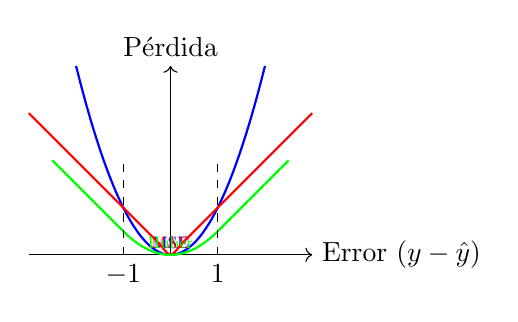
\begin{tikzpicture}[scale=0.6]
                    \draw[->] (-3,0) -- (3,0) node[right] {Error ($y - \hat{y}$)};
                    \draw[->] (0,0) -- (0,4) node[above] {Pérdida};
                    \draw[scale=1, domain=-2:2, smooth, variable=\x, blue, thick] plot ({\x}, {\x*\x}) node[above, pos=0.8, color=blue] {MSE};
                    \draw[scale=1, domain=-3:3, smooth, variable=\x, red, thick] plot ({\x}, {abs(\x)}) node[above, pos=0.8, color=red] {MAE};
                    \def\delta{1}
                    \draw[scale=1, domain=-\delta:\delta, smooth, variable=\x, green, thick] plot ({\x}, {0.5*\x*\x});
                    \draw[scale=1, domain=\delta:2.5, smooth, variable=\x, green, thick] plot ({\x}, {\delta*abs(\x) - 0.5*\delta*\delta}) node[above, pos=0.7, color=green] {Huber};
                    \draw[scale=1, domain=-2.5:-\delta, smooth, variable=\x, green, thick] plot ({\x}, {\delta*abs(\x) - 0.5*\delta*\delta});
                    \draw[dashed] (\delta, 0) node[below]{$\delta$} -- (\delta, 2);
                    \draw[dashed] (-\delta, 0) node[below]{$-\delta$} -- (-\delta, 2);
                \end{tikzpicture}
               % \caption{Visualización de pérdidas de regresión.}
            \end{figure}
        \end{column}
    \end{columns}
\end{frame}

\begin{frame}
	\frametitle{Negativo Logaritmo Verosimilitud (NLL) Regresión}
	%\framesubtitle{De la Predicción Puntual a la Distribución de Probabilidad}
\begin{columns}[T]
		\begin{column}{.5\textwidth}
    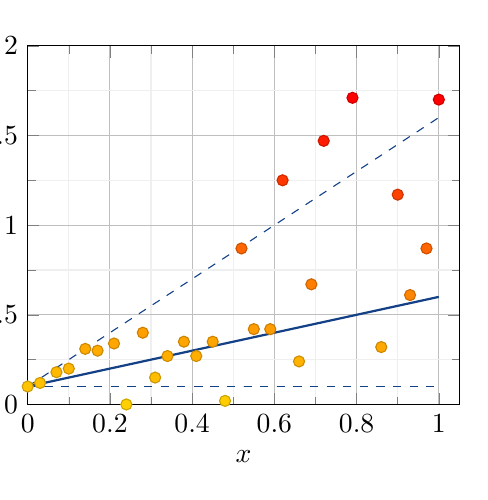
\begin{tikzpicture}[baseline,trim axis left]
    \begin{axis}[
       scale=0.8,
        xmin=0, xmax=1.05,
        ymin=0, ymax=2.0,
        xlabel={$x$},
        ylabel={$y$},
        grid=both,
        minor tick num=1,
        major grid style={lightgray},
        minor grid style={lightgray!25},
    ]
        \addplot+ [
            scatter, only marks
        ] coordinates {
    (0.0, 0.1) (0.03, 0.12) (0.07, 0.18) (0.1, 0.2) (0.14, 0.31) (0.17, 0.3) (0.21, 0.34) (0.24, -0.0) (0.28, 0.4) (0.31, 0.15) (0.34, 0.27) (0.38, 0.35) (0.41, 0.27) (0.45, 0.35) (0.48, 0.02) (0.52, 0.87) (0.55, 0.42) (0.59, 0.42) (0.62, 1.25) (0.66, 0.24) (0.69, 0.67) (0.72, 1.47) (0.76, -1.03) (0.79, 1.71) (0.83, -1.44) (0.86, 0.32) (0.9, 1.17) (0.93, 0.61) (0.97, 0.87) (1.0, 1.7)
        };
        \addplot [thick,
            mitblue,
            domain=0:1,
            samples=60,
        ]
            {0.5*x+0.1};
        \addplot [dashed,
            mitblue,
            domain=0:1,
            samples=60,
        ]
            {0.5*x+0.1+x};
            
              \addplot [dashed,
            mitblue,
            domain=0:1,
            samples=60,
        ]
            {0.5*x+0.1-0.5*x};  
    \end{axis}
    \end{tikzpicture}
    \end{column}
		\begin{column}{.5\textwidth}
     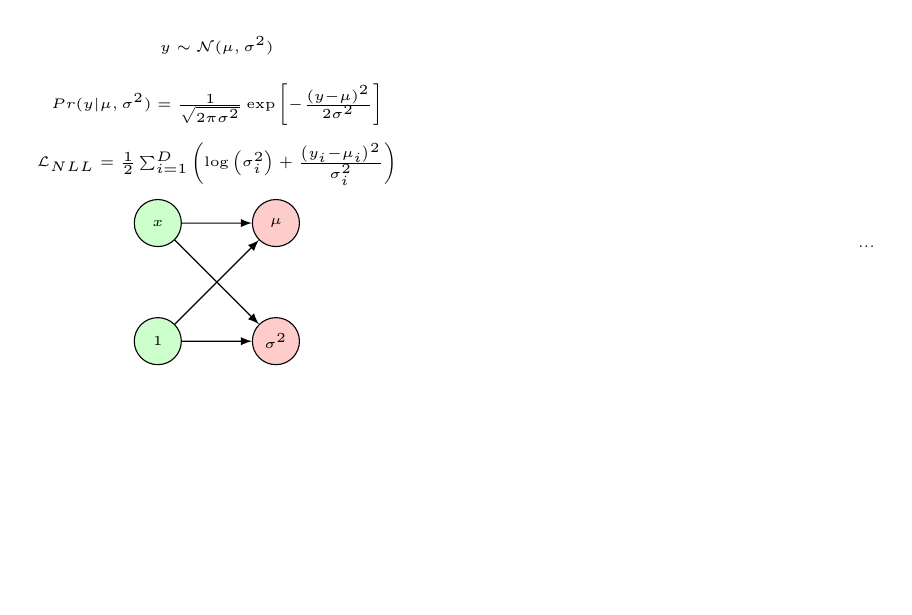
\begin{tikzpicture}[baseline,scale=1.5,font=\tiny]
			% Input Layer
			%\foreach \i in {1,...,2}
			\node[input] (I-1) at (0,-1-0.5) {$x$};
			\node[input] (I-2) at (0,-2-0.5) {$1$};
			%\node[below of=I-3, node distance=0.8cm] {Entradas};
			%\node (label1) at (0,-3.5) {Entradas};
			
			% Output Layer
			%\foreach \i in {1,...,2}
			%\node[output] (O-\i) at (1,-\i-0.5) {$y_{\i}$};
			\node[output] (O-1) at (1,-1-0.5) {$\mu$};
			\node[output] (O-2) at (1,-2-0.5) {$\sigma^2$};
			%\node[below of=O-2, node distance=0.8cm] {Salidas};
			%\node (label2) at (1,-3.5) {Salidas};
			\node at (6,-1.7) {...}; % Elipsis
			\node at (6,-4.5) {}; % Spacing hack
			\node at (0.5,0.0)  {$y \sim \mathcal N(\mu,\sigma^2)$};
			\node at (0.5,-0.5)  {$Pr(y|\mu, \sigma^2) = \frac{1}{\sqrt{2\pi\sigma^2}} \exp\left[-\frac{(y - \mu)^2}{2\sigma^2}\right] $};
			\node at (0.5,-1.0)  {$\mathcal{L}_{NLL} = \frac{1}{2}\sum_{i=1}^D \left(\log\left(\sigma_i^2\right) + \frac{\left(y_i - \mu_i\right)^2}
        {\sigma^2_i}\right)$};
			% Connections
			\foreach \i in {1,...,2}
			\foreach \j in {1,...,2}
			\draw[line] (I-\i) -- (O-\j);
		\end{tikzpicture}

	\end{column}
	\end{columns}


\end{frame}

% --- Sección 3: Pérdidas de Clasificación ---
\section{Funciones de Pérdida para Clasificación}

\begin{frame}{Pérdidas de Clasificación Probabilísticas}
    \begin{block}{Entropía Cruzada (Cross-Entropy)}
        Es la función de pérdida estándar para tareas de clasificación. Mide la divergencia entre la distribución de probabilidad predicha y la distribución verdadera (one-hot).
        
        \textbf{Binaria (BCE):} Para dos clases.
        $$ \mathcal{L}_{BCE} = -[y \log(\hat{p}) + (1-y) \log(1-\hat{p})] $$
        
        \textbf{Categórica (CCE):} Para múltiples clases.
        $$ \mathcal{L}_{CCE} = - \sum_{j=1}^{C} y_j \log(\hat{p}_j) $$
    \end{block}
    
%    \begin{alertblock}{Problema: Desbalance de Clases}
%        Si una clase domina el conjunto de datos, el modelo puede minimizar la pérdida simplemente prediciendo siempre esa clase. Esto lleva a un rendimiento pobre en las clases minoritarias.
%    \end{alertblock}
\end{frame}

\begin{frame}
	\frametitle{Negativo Logaritmo Verosimilitud (NLL) Clasificación}
	%\framesubtitle{De la Predicción Puntual a la Distribución de Probabilidad}
\begin{columns}[T]
		\begin{column}{.5\textwidth}
    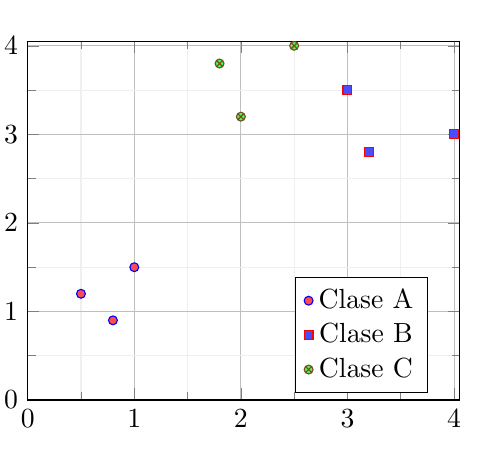
\begin{tikzpicture}[baseline,trim axis left]
        \begin{axis}[
            scale=0.8,
        xmin=0, xmax=4.05,
        ymin=0, ymax=4.05,
        %xlabel={$x_1$},
        %ylabel={$x_2$},
        grid=both,
        minor tick num=1,
        major grid style={lightgray},
        minor grid style={lightgray!25}, legend style={at={(0.62,0.02)},anchor=south west}       ]
        % Class 1
        \addplot+[only marks, mark options={fill=red!70, scale=0.8}] coordinates
      { (0.5,1.2)  (1.0,1.5) (0.8,0.9)};
        \addlegendentry{Clase A}
	\addplot+[only marks, mark options={fill=blue!70, scale=0.8}] coordinates
      { (3.0,3.5)  (3.2,2.8) (4.0,3.0)};
      \addlegendentry{Clase B}
      \addplot+[only marks, mark options={fill=green!70, scale=0.8}] coordinates
      { (1.8,3.8)  (2.5,4.0) (2.0,3.2)};
      \addlegendentry{Clase C}
      
        \end{axis}
    \end{tikzpicture}
    \end{column}
		\begin{column}{.5\textwidth}
 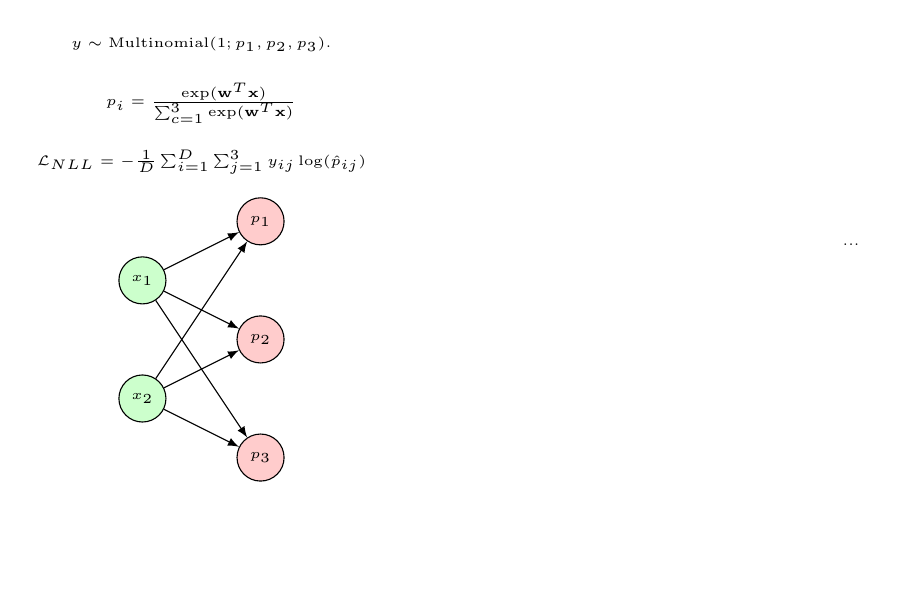
\begin{tikzpicture}[baseline,scale=1.5,font=\tiny]
			% Input Layer
			%\foreach \i in {1,...,2}
			\node[input] (I-1) at (0,-1.5-0.5) {$x_1$};
			\node[input] (I-2) at (0,-2.5-0.5) {$x_2$};
			%\node[below of=I-3, node distance=0.8cm] {Entradas};
			%\node (label1) at (0,-3.5) {Entradas};
			
			% Output Layer
			%\foreach \i in {1,...,2}
			%\node[output] (O-\i) at (1,-\i-0.5) {$y_{\i}$};
			\node[output] (O-1) at (1,-1-0.5) {$p_1$};
			\node[output] (O-2) at (1,-2-0.5) {$p_2$};
			\node[output] (O-3) at (1,-3-0.5) {$p_3$};
			%\node[below of=O-2, node distance=0.8cm] {Salidas};
			%\node (label2) at (1,-3.5) {Salidas};
			\node at (6,-1.7) {...}; % Elipsis
			\node at (6,-4.5) {}; % Spacing hack
			\node at (0.5,0.0)  {$y \sim \text{Multinomial}(1; p_{1}, p_{2},  p_{3}).$};
			\node at (0.5,-0.5)  {$p_i = \frac{\exp(\mathbf w^T \mathbf x)}{\sum_{c=1}^3 \exp (\mathbf w^T \mathbf x)} $};
			\node at (0.5,-1.0)  {$\mathcal{L}_{NLL} =- \frac{1}{D}\sum_{i=1}^D \sum_{j=1}^{3} y_{ij} \log(\hat{p}_{ij})$};
			% Connections
			\foreach \i in {1,...,2}
			\foreach \j in {1,...,3}
			\draw[line] (I-\i) -- (O-\j);
		\end{tikzpicture}
	\end{column}
	\end{columns}


\end{frame}

\begin{frame}{Desbalance de Clases}
    \begin{block}{Entropía Cruzada Ponderada (Weighted Cross-Entropy)}
        Asigna un peso mayor a la pérdida de las clases minoritarias. Es una solución simple y efectiva.
        $$ \mathcal{L}_{WCE} = - \sum_{j=1}^{C} \alpha_j y_j \log(\hat{p}_j) $$
        donde $\alpha_j$ es inversamente proporcional a la frecuencia de la clase $j$.
    \end{block}

    \begin{block}{Pérdida Focal (Focal Loss)}
        Una mejora sobre WCE que añade un factor de modulación para reducir la contribución de los ejemplos "fáciles" (bien clasificados).
        $$ \mathcal{L}_{FL} = -(1-p_t)^\gamma \log(p_t) $$
        Esto fuerza al modelo a centrarse en los ejemplos difíciles, que a menudo pertenecen a las clases minoritarias.
    \end{block}
\end{frame}
%
%% --- Sección 4: Pérdidas en Visión por Computadora ---
\section{Pérdidas en Visión por Computadora}

\begin{frame}[shrink]{Detección de Objetos: Un Problema Compuesto}
    La detección de objetos es una tarea multi-objetivo que requiere:
    \begin{enumerate}
        \item \textbf{Clasificación:} ¿Qué objeto hay en la caja?
        \item \textbf{Localización:} ¿Dónde está la caja (bounding box)?
    \end{enumerate}
\centering
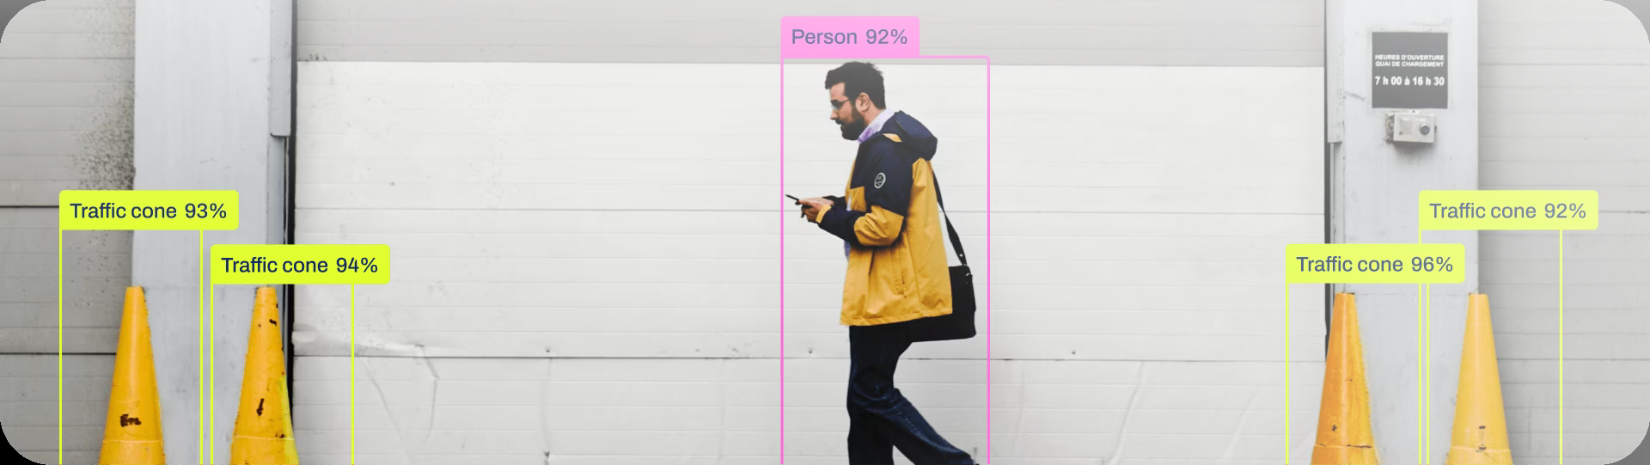
\includegraphics[width=0.8\textwidth]{figures/object-detection-examples} 
 
        \begin{block}{Pérdida Compuesta}
        La función de pérdida total es una suma ponderada de una pérdida de clasificación y una pérdida de regresión.
        $$ \mathcal{L}_{total} = \mathcal{L}_{cls} + \lambda \mathcal{L}_{reg} $$
    \end{block}
    
    \begin{itemize}
        \item $\mathcal{L}_{cls}$ suele ser Entropía Cruzada o Focal Loss.
        \item $\mathcal{L}_{reg}$ se especializa en la regresión de las coordenadas de la caja.
    \end{itemize}
\end{frame}

\begin{frame}[shrink]{Pérdidas para la Regresión de Bounding Box}
    \begin{block}{Smooth L1 Loss}
        Una variante de la pérdida de Huber, es el estándar de facto en muchos detectores de dos etapas como Faster R-CNN. Es robusta a outliers pero suave cerca de cero.
    \end{block}
    
    \begin{block}{Pérdidas basadas en IoU (Intersection over Union)}
        Optimizan directamente la métrica de evaluación principal: el solapamiento entre la caja predicha ($B_p$) y la real ($B_t$).
        $$ \text{IoU} = \frac{\text{Area}(B_p \cap B_t)}{\text{Area}(B_p \cup B_t)} \quad \implies \quad \mathcal{L}_{IoU} = 1 - \text{IoU} $$

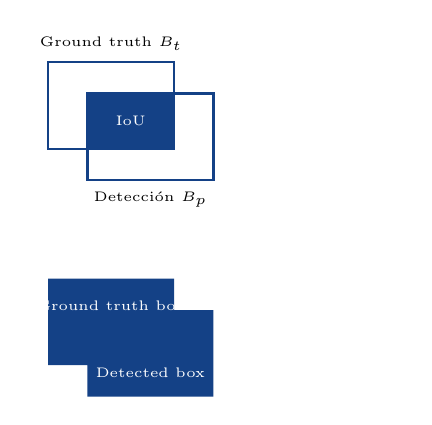
\begin{tikzpicture}[
   scale=0.5,
    % Use a sans-serif font, slightly bold to match the image
    font=\tiny,
    % Define a style for the hollow bounding boxes
    box/.style={draw=mitblue, thick},
    % Define a style for the larger formula text
    %formula_text/.style={scale=1.3}
]

% --- LEFT SIDE: TEXT FORMULA ---
% --- RIGHT SIDE: DIAGRAMS ---
% Define a central point for the diagrams to make positioning easier
\coordinate (diagram_center) at (5.25, 0);

% --- NUMERATOR: Intersection Diagram ---
\begin{scope}[shift={(diagram_center)}, yshift=2.8cm]
    % Define coordinates for the two boxes
    \coordinate (gt_bl) at (-2.2, -1);   % Ground Truth Bottom-Left
    \coordinate (gt_tr) at (1, 1.2);      % Ground Truth Top-Right
    \coordinate (dt_bl) at (-1.2, -1.8);  % Detected Bottom-Left
    \coordinate (dt_tr) at (2, 0.4);      % Detected Top-Right

    % Calculate the coordinates of the intersection rectangle
    \coordinate (int_bl) at (-1.2, -1);   % max(x_gt, x_dt), max(y_gt, y_dt)
    \coordinate (int_tr) at (1, 0.4);     % min(x_gt, x_dt), min(y_gt, y_dt)

    % Draw the filled intersection area first
    \fill[mitblue] (int_bl) rectangle (int_tr);
    
    % Draw the hollow bounding boxes on top so their outlines are visible
    \draw[box] (gt_bl) rectangle (gt_tr);
    \draw[box] (dt_bl) rectangle (dt_tr);

    % Add labels for the boxes and the intersection
    \node[anchor=south] at (-0.6, 1.25) {Ground truth $B_t$};
    \node[anchor=north] at (0.4, -1.85) {Detección $B_p$};
    \node[white] at (-0.1, -0.3) {IoU};

\end{scope}
     %
% --- DENOMINATOR: Union Diagram ---
\begin{scope}[shift={(diagram_center)}, yshift=-2.7cm]
    % Use the same box coordinates as the numerator for consistency
    \coordinate (gt_bl) at (-2.2, -1);
    \coordinate (gt_tr) at (1, 1.2);
    \coordinate (dt_bl) at (-1.2, -1.8);
    \coordinate (dt_tr) at (2, 0.4);

    % Draw the union shape by filling a single path that outlines the two boxes
    % The path follows the outer perimeter of the combined shape
    \fill[mitblue] (gt_bl) -- 
                  (-2.2, 1.2) -- % Top-left of GT
                  (1, 1.2) --   % Top-right of GT
                  (1, 0.4) --
                  (2, 0.4) --   % Top-right of Detected
                  (2, -1.8) --  % Bottom-right of Detected
                  (-1.2, -1.8) --% Bottom-left of Detected
                  (-1.2, -1) --
                  cycle;

    % Add labels inside the union shape
    \node[white] at (-0.6, 0.5) {Ground truth box};
    \node[white] at (0.4, -1.2) {Detected box};
    \node[inner sep=0pt] (bbox) at (6.8,2.5) {   };
\end{scope}

\end{tikzpicture}


    \end{block}
\end{frame}

\begin{frame}{Reconocimiento Facial: Aprendizaje Métrico}
    El objetivo no es solo clasificar, sino aprender un \textbf{espacio de embedding} donde:
    \begin{itemize}
        \item Las distancias \textbf{intra-clase} (entre caras de la misma persona) sean pequeñas.
        \item Las distancias \textbf{inter-clase} (entre caras de personas diferentes) sean grandes.
    \end{itemize}
    
    \begin{block}{Pérdidas Basadas en Margen Angular}
        En lugar de optimizar logits, estas pérdidas operan directamente sobre el ángulo entre el embedding de una cara y el vector prototipo de su clase.
        \begin{itemize}
            \item \textbf{CosFace:} Introduce un margen aditivo en el espacio del coseno.
            \item \textbf{ArcFace:} Introduce un margen aditivo directamente en el ángulo.
        \end{itemize}
    \end{block}
\end{frame}

\begin{frame}{Pérdida de Triplete (Triplet Loss)}
    Una pérdida clásica de aprendizaje métrico que no requiere un número fijo de clases.
    
    \begin{block}{Formulación}
        Se consideran tres ejemplos: un \textbf{ancla} ($A$), un \textbf{positivo} ($P$, misma identidad) y un \textbf{negativo} ($N$, identidad diferente). La pérdida busca que la distancia del ancla al positivo sea menor que la distancia al negativo, por un margen $\alpha$.
        $$ \mathcal{L}_{Triplet} = \max\left(0, \underbrace{\|f(A) - f(P)\|_2^2}_{\text{distancia positiva}} - \underbrace{\|f(A) - f(N)\|_2^2}_{\text{distancia negativa}} + \alpha\right) $$
    \end{block}
    
\end{frame}

\section{Conclusión}

\begin{frame}{Conclusiones}
    \begin{itemize}
        \item La elección de la función de pérdida es una decisión de diseño fundamental que define el objetivo de la optimización y tiene un impacto directo en el rendimiento del modelo.
        
        \item No existe una "bala de plata". La pérdida ideal depende de la tarea (\textbf{regresión}, \textbf{clasificación}), las características de los datos (\textbf{outliers}, \textbf{desbalance}) y la métrica de evaluación final.
        
        \item Tareas complejas como la \textbf{detección de objetos} o el \textbf{reconocimiento facial} han impulsado el desarrollo de pérdidas especializadas (basadas en IoU, aprendizaje métrico) que van más allá de las formulaciones estándar.
        
        \item El futuro de la investigación se dirige hacia la \textbf{búsqueda automatizada} de funciones de pérdida y el diseño de objetivos que incorporen \textbf{robustez, interpretabilidad y equidad}.
    \end{itemize}
\end{frame}
\end{document}
